\section{Разработка архитектуры наземной станции}
Аппаратная часть наземной станции состоит из:
\begin{itemize}
	\item компьютера;
	\item передающего модуля радиоуправления;
	\item видеоприемника;
	\item устройства приема-передачи телеметрии.
\end{itemize}

Наземная станция должна обмениваться телеметрией с квадрокоптером, получать видеопоток с квадрокоптера, и отправлять управляющий сигнал в виде команд MAVROS. Чем больше бод -- рейт подключенных модулей и меньше задержка сигнала, тем быстрее осуществляется выполнение команд. Для устройств приема-передачи телеметрии рекомендуется бод -- рейт, равный 921600. Учитывая эти факторы, выбираются устройства телеметрии и видеоприемник.
К компьютеру по UART порту подключается модуль радиоуправления и устройство приема-передачи телеметрии. Через USB порт подключается видеоприемник. Настраиваем видеоприемник на диапазон частот, соответствующий частотам видеопередатчика квадрокоптера и переходим к программной части.

Для позиционирования робототехнических систем с помощью компьютерного зрения используются aruco маркеры -- квадратные маркеры, состоящий из широкой черной границы и внутренней двоичной матрицы, которая определяет его идентификатор (id). Черная рамка облегчает ее быстрое обнаружение на изображении, а двоичная кодификация позволяет ее идентифицировать \cite{opencv}.

В ходе исследования был найден пакет aruco\_gridboard, предназначенный для работы с aruco-маркерами. Образ clover, который предоставляет пакеты и инструменты для позиционирования и управления квадрокоптером на базе ROS по MAVROS. Образ clover подходит для выполнения поставленной задачи.

Программная часть представляет собой совокупность взаимодействущего программного обеспечения, включающего в себя:
\begin{itemize}
	\item операционную систему на базе ядра linux;
	\item пакет clover;
	\item qgroundcontrol.
\end{itemize}

В qgroundcontrol выставляется бод -- рейт. Далее происходит подключение и обмен данными с устройством приема-передачи телеметрии, расположенного на борту квадрокоптера.
По MAVLink протоколу передаются данные в указанный UART, и все программы, прослушивающие этот UART, порт имеют доступ к данным с борта квадрокоптера. Для взаимодействия через ROS инструменты необходима настройка всех параметров подключения. На данном этапе НИР используется готовой решение от Copter Express -- пакет clover, позволяющий производить настройку максимально просто. В launch файлах пакета прописываются все параметры. Указывается UART, бауд -- рейт, и в консоли запускается clover с помощью команд, представленных в листинге \ref{lst:45}:
\begin{Program}[H]
	\caption{Запуск clover} \label{lst:45}
	\begin{MyCode}
	gs@groundstation:~$ source /home/clover/catkin\_ws/devel/setup.bash
	gs@groundstation:~$ roslaunch clover clover.launch
	\end{MyCode}
\end{Program}

После этого доступны все инструменты clover. На листинге \ref{lst:5} приведен результат выполнения команды для получения телеметрии. "frame\_id: ''" означает, что показания берутся в системе координат относительно квадрокоптера.
\begin{Program}[H]
	\caption{Вывод телеметрии квадрокоптера в консоли} \label{lst:5}
	\begin{MyCode}
	gs@groundstation:~$ rosservice call /get_telemetry "frame_id: ''" 
	frame_id: "map"
	connected: True
	armed: False
	mode: "MANUAL"
	x: -0.00260298536159
	y: -6.72723326716e-05
	z: 0.00103790743742
	lat: 0.0
	lon: 0.0
	alt: 0.0
	vx: -0.00717502878979
	vy: -0.00176917202771
	vz: 0.00364218326285
	pitch: 0.0221049506217
	roll: -0.0172985047102
	yaw: 0.000302107335301
	pitch_rate: 0.00245076417923
	roll_rate: 0.00449034944177
	yaw_rate: 0.00266480189748
	voltage: 12.1499996185
	cell_voltage: 4.05000019073
	gs@groundstation:~$
	\end{MyCode}
\end{Program}

Видеоприемник подключен в порт /dev/video0. Он указывается в launch-файле, далее перезагружается clover и проверяются в web-браузере топики по адресу localhost:8080 (рисунок \ref{fig:topic}).

\begin{figure}[H]
	\centering
	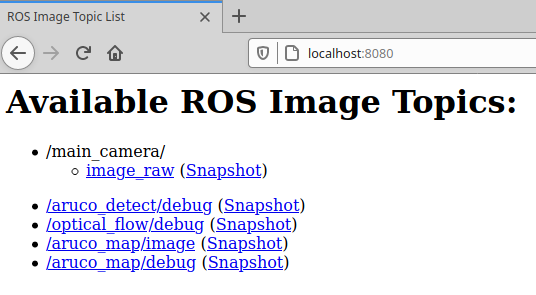
\includegraphics[width=0.5\linewidth]{../RW/pics/topic}
	\caption{Список топиков, доступный по умолчанию
	}
	\label{fig:topic}
\end{figure}

Список НОД также меняется в launch файлах. В image raw топике будет отображаться видеопоток, полученный видеоприемником с борта квадрокоптера, в остальных топиках публикуются:
\begin{itemize}
	\item aruco-detect (на image raw определяются с помощью openCV aruco маркеры);
	\item optical flow (на изображение с image raw накладывается точка отсчета для лазерного дальномера);
	\item aruco map (карта маркеров, прописанная в конфигурационном файле).
\end{itemize}

Optical flow отключается, так как на БПЛА не установлен лазерный дальномер.
\subsection{Конфигурация наземной станции}
Наземная станция представляет собой компьютер, подключенный к тому же роутеру, что и дрон. Операционная система на базе ядра linux, установлены пакеты ros, соответствующие версии ОС, в данном случае ros-melodic-full, и gstreamer для приема видеопотока.

\subsection{Настройка mavros}
Для того, чтобы ноды могли обмениваться данными, необходим roscore \cite{pkg}. roscore - это набор нод и программ, которые являются предпосылками системы на основе ROS \cite{ros}. Запускается с помощью команды \$ roscore в одной из вкладок консоли, однако при использовании roslaunch это действие необязательно -- при выполнении roslaunch первым делом запускается roscore.

roslaunch - это инструмент для простого запуска нескольких нод ROS. Он включает в себя опции для автоматического запуска уже завершенных процессов. roslaunch принимает один или несколько файлов конфигурации XML (с расширением .launch ), определяющих параметры, которые необходимо установить, и ноды для запуска, а также машины, на которых они должны запускаться \cite{ros}.

Для получения телеметрии полетного контроллера в /opt/ros/melodic/sha\-re/mavros/launch/px4.launch файле поменять параметры fcu\_url, указав нужный адрес и порт. Видеопоток планируется получать UDP пакетами, для их обработки необходимо указать адрес и порт в параметре gcs\_url (листинг \ref{lst:9}):
\begin{Program}[H]
	\caption{Измененные параметры в launch файле mavros} \label{lst:9}
	\begin{MyCode}
	<arg name="fcu_url" default="tcp://192.168.1.148:2000?ids=1,240"/>   
	<arg name="gcs_url" default="udp://@127.0.0.1:14555"/>
	\end{MyCode}
\end{Program}

\subsection{Подготовка инструментов для получения и обработки видеопотока}
Для получения трансляции и публикации топиков с изображением с камеры используется gscam. Он собирается из репозитория \url{https://github.com/ros-drivers/gscam} командами, представленными в листинге \ref{lst:10}:
\begin{Program}[H]
	\caption{Сборка gscam} \label{lst:10}
	\begin{MyCode}
	$ git clone https://github.com/ros-drivers/gscam
	$ cd gscam
	$ cmake -DGSTREAMER_VERSION_1_x=On
	$ сmake install
	\end{MyCode}
\end{Program}

Распознавание карты aruco маркеров на изображении, получаемом из топиков gscam, и публикацию полученных координат в топик /vision/pose производит aruco\_gridboard. Команды для сборки этого пакета представлены в листинге \ref{lst:11}:
\begin{Program}[H]
	\caption{Сборка aruco\_gridboard} \label{lst:11}
	\begin{MyCode}	
	$ cd ~/catkin_ws/src
	$ git clone https://github.com/anbello/aruco_gridboard.git
	$ cd ..
	$ catkin_make
	$ source devel/setup.bash
	$ catkin_make --only-pkg-with-deps aruco_gridboard
	\end{MyCode}
\end{Program}

Проделанных шагов достаточно, чтобы на наземной станции отобразить положение дрона относительно карты маркеров.